%%%% SEITENRAENDER, SCHRIFTGROESSE UND ZEILENABSTAND NICHT ABAENDERN => SONST GIBT ES PUNKTEABZUG
\documentclass[a4paper,11pt,singlespacing]{article}
% \usepackage[left=2.5cm,right=2.5cm,top=2.5cm]{geometry}
\usepackage{setspace}
\usepackage[utf8]{inputenc}
\usepackage[T1]{fontenc}
\usepackage{graphicx}
\usepackage[ngerman]{babel}
\usepackage{color}
\usepackage{wrapfig}
\usepackage{titleref}
\usepackage{hyperref}
\usepackage[rightcaption]{sidecap}
\usepackage{listings,xcolor}
\usepackage[numbers,round]{natbib}
\usepackage{float} % For image floating ([H] -> "here")

% Configuration
\sloppy
\setlength{\parindent}{0ex} % Absatzeinrückung verhindern
\graphicspath{ {images/} }

\begin{document}
\pagenumbering{roman}

% Cover
\title{Systemadministration - Mailserver Honeypot zum analysieren von Spam}
\author{Manuel Adams 27470, Michael Ruf 27428, Mario Waizenegger 29608}
\maketitle
\begin{abstract}
Heutzutage wird viel \nameref{itm:Spam} verschickt. Einiges davon wird erkannt und gefiltert.
Um die Analyse von Spam-Nachrichten und deren Versender zu ermöglichen, wird ein Mailserver \nameref{itm:Honeypot} aufgesetzt.
Dieser soll \nameref{itm:Spam}-Nachrichten erhalten können, sowie als offener Verteiler für Spammer verfügbar sein.
\end{abstract}

\newpage

% Table of contents
\tableofcontents

\newpage
\pagenumbering{arabic}

% Content
\section{Einleitung}\label{sec:Einleitung}
	% NOTE "Wir" erlaubt
	Warum \nameref{itm:Spam} versandt wird ist vielen Menschen ein Rätsel.
	Das wirft die Fragen auf, wer Spam versendet und was die Beweggründe von Spammern sind.
	Wie geht man mit Spam um und was passiert wenn man auf \nameref{itm:Spam} reagiert?
	Ein \nameref{itm:Spam} \nameref{itm:Honeypot} bietet die Möglichkeit diese Fragen zu analysieren und die nötigen Daten zu erheben.
	% NOTE Warum lohnt sich das?
	\\
	Da die Methoden von erfolgreichen Spammern nicht dokumentiert sind, ist das Bekanntmachen des "`\nameref{itm:OpenRelay}"'"~Servers schwierig.
	Zudem ist es zeitaufwendig die eigenen Mail-Adressen unter Spammern bekannt zu machen und viele authentische Spam-Mails in kurzer Zeit zu erhalten eine Herausforderung.
	% NOTE Man kann man beim Ergebnis nochmal Stellungnahme hierzu nehmen oder den Text hier ergänzen
	% -----
	% - Wirtschaftlichkeit
	% - Andere Beweggründe
	% - Findet man Informationen über Systeme, von denen Spam verschickt wird?
	% - Werden die Nachrichten generiert? (Bots)

	\subsection{Ziel der Arbeit}\label{sec:EinleitungZiel}
		Es soll durch einen Mailserver Honeypot Erkenntnisse über Herkunft, Zweck und Zielgruppe von \nameref{itm:Spam} Nachrichten erhalten werden.
		Zusätzlich soll erarbeitet werden welche weiteren nützlichen Informationen man den Mails entnehmen kann.
		Durch diese Informationen soll die Motivation von Spammern besser verstanden und entsprechende Vorkehrungen zum Schutz ermöglicht werden.
		% NOTE Was wird genau analysiert
	
	\subsection{Vorgehensweise}\label{sec:EinleitungVorgehensweise}
		Um den Honeypot zu realisieren muss der Mail-Dienst aus dem Internet zugänglich sein.
		Dieser besteht hierbei aus Ausgangsserver und Eingangsserver.
		Hierzu werden auf einer \nameref{itm:VirtuelleMaschine} die Dienste in \nameref{itm:Container}n aufgesetzt.
		Aus Sicherheitsgründen muss die VM ins interne Netz abgeschottet sein.
		Der Aufbau ist in \autoref{fig:Hierarchy} visualisiert.

		\begin{figure}[H]
		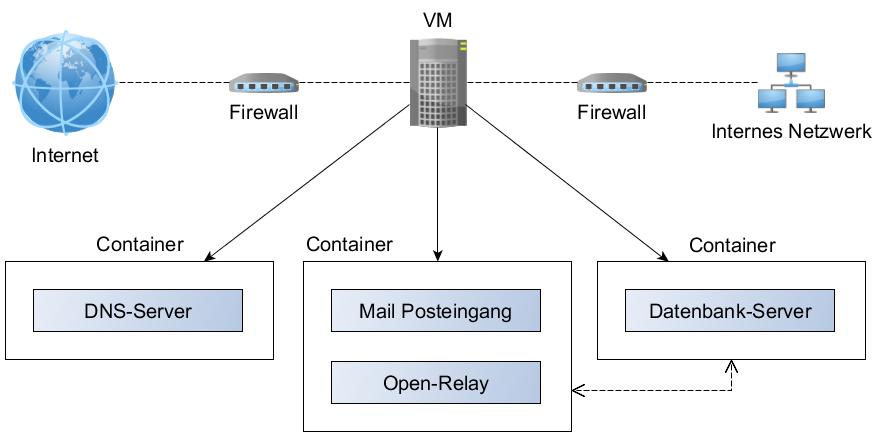
\includegraphics[width=\linewidth]{2-Hierarchy.png}
		\caption{Netzwerkstruktur}
		\label{fig:Hierarchy}
		\end{figure}

		Um den Eingangsserver zu realisieren sind folgende Aufgaben erforderlich:
		\begin{enumerate}
		\item Mail Eingangsserver bereitstellen und konfigurieren
		\item \nameref{itm:DNS} Server einrichten um realistische E-Mail-Adressen bereitzustellen
		\item Bei möglichst vielen Diensten mit unterschiedlichen Mailadressen registrieren
		\item Mails analysieren
		\end{enumerate}

		Den Ausgangsserver betreffend sind folgende Aufgaben erforderlich:
		\begin{enumerate}
		\item Mail Ausgangsserver bereitstellen und konfigurieren
		\item Als "`\nameref{itm:OpenRelay}"' im Internet durchsickern lassen
		\item Eingehende Mails tatsächlich weiterleiten
		\item Mails analysieren
		\end{enumerate}

	\subsection{Aufbau der Arbeit}\label{sec:EinleitungAufbau}
%		% Hier geht es wirklich um den Aufbau der wissenschaftlichen Arbeit, nicht um das Projekt
%		In Abschnitt 2 geht es um..
%		In Abschnitt 3 geht es um..
%		TODO


\section{Grundbegriffe}\label{sec:Grundbegriffe}
	Die folgenden Begriffsdefinitionen und Unterscheidungen sind zum einen zur Verdeutlichung, wie Begriffe in dieser Arbeit verstanden werden und um Fachbegriffe zu erklären.
	
	% NOTE Alle nochmal durchnudeln
	\begin{description}
	\item[Spam\label{itm:Spam}]\hfill \\
		Als Spam oder Junk werden unerwünschte, in der Regel auf elektronischem Weg übertragene Nachrichten (Informationen) bezeichnet, die dem Empfänger unverlangt zugestellt werden und häufig werbenden Inhalt enthalten. Dieser Vorgang wird Spamming oder Spammen genannt, der Verursacher Spammer.\cite{Spam}
	\item[Honeypot\label{itm:Honeypot}]\hfill \\
		Sicherheitstechnisch scheinbar verwundbares Computerprogramm, das Computerviren, -würmer und Trojaner anlockt, um sie zu registrieren und unschädlich zu machen.\cite{Honeypot}
	\item[Open-Relay\label{itm:OpenRelay}]\hfill \\
		Ein SMTP-Relay-Server der durch unzureichende Sicherheitskonfiguration auch Mails weiterleitet bei denen er weder für die Absender- noch für die Zieladresse zuständig ist, wird als "`Open relay"' bezeichnet.\cite{SMTP-Relay-Server}
	\item[Virtuelle Maschine (VM)\label{itm:VirtuelleMaschine}]\hfill \\
		Eine VM ist eine Kapselung eines Rechnersystems auf Softwareebene. Dadurch lässt sich eine Rechnerarchitektur in einem Container simulieren. \cite{VM}
	\item[Blacklist \label{itm:Blacklist}]\hfill \\
		Eine Blacklist oder "`schwarze Liste"' enthält eine Auflistung von Daten, die von einem Prozess ausgeschlossen werden solle. Das Gegenteil dazu ist eine Whitelist. \cite{Blacklist}
	\item[Container\label{itm:Container}]\hfill \\
		Containervirtualisierung ist eine Methode, um mehrere Instanzen eines Betriebssystems isoliert voneinander auf einem Hostsystem zu betreiben.\cite{Container}
	\item[DNS\label{itm:DNS}]\hfill \\
		Das Domain Name System (DNS) ist einer der wichtigsten Dienste in vielen IP-basierten Netzwerken. Seine Hauptaufgabe ist die Beantwortung von Anfragen zur Namensauflösung.\cite{DNS}
	\item[DKIM\label{itm:DKIM}]\hfill \\
		DKIM (DomainKeys Identified Mail) ist eine Methode der E-Mail-Authentifizierung. DKIM fügt Ihren Mails eine Signatur hinzu, die Ihrer Domain zugeordnet ist und bei allen ausgehenden E-Mails genutzt wird. Das Verwenden eines DomainKey ist eine Technik (ähnlich wie SPF), die das Fälschen des Absenders einer E-Mail erschweren soll.\cite{DKIM}
	\item[Hook\label{itm:Hook}]\hfill \\
		Hook (englisch für Haken, auch Einschubmethode genannt) bezeichnet in der Programmierung eine Schnittstelle, mit der fremder Programmcode in eine bestehende Anwendung integriert werden kann, um diese zu erweitern, deren Ablauf zu verändern oder um bestimmte Ereignisse abzufangen.\cite{Hook}
	\item[Catch-All-Mail-Adressen\label{itm:Catch-All-Mail}]\hfill \\
		Ein Catch-All-e-Mail-Konto ist eine Adresse, die alle Nachrichten mehr erhalten möchten, die an eine falsche e-Mail-Adresse für eine Domain adressiert sind angegeben ist.\cite{Catch-All-Mail}
	\end{description}


\section{Problemstellung}\label{sec:Problemstellung}
	Spammer dokumentieren ihre Arbeit eher nicht.
	Daher sind deren Vorgehensweisen unklar.
	Um einen Einblick zu erhalten sind nachfolgende Probleme zu lösen.
	% Unterpunkte:
	% - Sehr konkret
	% - Forschungsfrage festnageln

	\subsection{Konfiguration}\label{sec:ProblemstellungKonfiguration}
		Um einen reibungslosen Ablauf zu gewährleisten muss der Mailserver in der Lage sein Mails zu empfangen.
		Empfangene Mails sollen persistiert werden.
		Eine hohe Verfügbarkeit ist hier von Vorteil.
		\\
		Der Server soll zudem als \nameref{itm:OpenRelay} dienen.
		Hierfür muss dieser so konfiguriert werden, dass eingehende externe Mails nicht abgewiesen werden.
		\\
		Um die Mails abzulegen bietet sich ein Datenbank Server an.
		Die Daten auf dem Mail-Server dürfen dadurch jederzeit verworfen werden und Änderungen am Mailserver können ohne Auswirkung auf vorhandene Daten umgesetzt werden.

	\subsection{Mail-Adressen verteilen}\label{sec:ProblemstellungMailsVerteilen}
		Damit authentische Spam Mails erhalten werden müssen die E-Mail-Adressen echt wirken.
		Um das zu erreichen müssen die Adressen
		\begin{itemize}
		\item möglichst lange, also möglichst früh in Verwendung sein,
		\item aktiv benutzt werden
		\item und bei möglichst vielen Diensten benutzt werden.
		\end{itemize}
		Es soll identifiziert werden können von welchem Dienst eine Mail eingeht.
		Zudem bietet es sich an auf eingehende Spam-Mails zu reagieren indem man bspw. auf vorhandene Links klickt, da Tracking-Links enthalten sein können oder auf die Mail antwortet. % TODO Def Tracking

	\subsection{Open-Relay Publizieren}\label{sec:ProblemstellungPublizieren}
		Der \nameref{itm:Honeypot} muss bei Spammern als unsicher wirkender \nameref{itm:OpenRelay} und guter Spamverteiler bekannt werden.
		Im Internet muss die Adresse des Servers hierzu so verteilt werden, dass Spammer darauf aufmerksam werden.
		Nach Möglichkeit sollte der Server nicht in einer \nameref{itm:OpenRelay} \nameref{itm:Blacklist} auftauchen, da er ansonsten nicht mehr nützlich für Spammer ist.

	\subsection{Analysieren}\label{sec:ProblemstellungAnalysieren}
		Es soll erarbeitet werden, welche Aspekte von Spam analysiert werden können:
		\begin{itemize}
		\item Kann man Informationen über das System von dem gesendet wurde erhalten?
		\item Könnte man den Weg den die \nameref{itm:Spam}"~Mails vom Versender bis zum Empfänger genommen haben zurückverfolgen?
		\item Inwiefern lässt sich der Inhalt der Mail auf Schreibweise, Textinhalt oder auch Anhänge analysieren?
		\end{itemize}


\section{Anforderungsanalyse}\label{sec:Anforderungsanalyse}
	Folgende Anforderungen \textbf{MÜSSEN}/\textbf{SOLLEN}/\textbf{KÖNNEN} erarbeitet werden, damit die \nameref{sec:Problemstellung} gelöst werden kann:

	\begin{itemize}
	\item
		Der Mail"~Server \textbf{MUSS} die Mails empfangen können.
		(\ref{sec:ProblemstellungKonfiguration})
	\item
		Es \textbf{MUSS} auf eingehende Spam"~Mails reagiert werden.
		(\ref{sec:ProblemstellungMailsVerteilen})
	\item
		Es \textbf{MUSS} erarbeitet werden, welche Aspekte von Spam analysiert werden können.
		(\ref{sec:ProblemstellungAnalysieren})
	\item
		Der Mail"~Server \textbf{SOLL} als \nameref{itm:OpenRelay} dienen.
		Diese Mails sollen nicht versendet, sondern lediglich persistiert werden.
		(\ref{sec:ProblemstellungKonfiguration})
	\item
		Die Mail"~Adressen \textbf{SOLLEN} echt wirken.
		(\ref{sec:ProblemstellungMailsVerteilen})
	\item
		Die Adresse des \nameref{itm:OpenRelay} Servers \textbf{SOLL} bei Spammern bekannt werden.
		(\ref{sec:ProblemstellungPublizieren})
	\item
		Die Daten \textbf{KÖNNEN} auf einem Datenbankserver abgelegt werden, welcher über Mail"~"`\nameref{itm:Hook}s"' die Daten bekommt.
		(\ref{sec:ProblemstellungKonfiguration})
	\item
		Zur Identifizierung \textbf{KANN} sich bei den Diensten mit einer "`\nameref{itm:Catch-All-Mail}"' mit einem Präfix für den jeweiligen Dienst registriert werden.
		(\ref{sec:ProblemstellungMailsVerteilen})
	\item
		Der Server \textbf{KÖNNTE} nicht in einer \nameref{itm:OpenRelay} \nameref{itm:Blacklist} auftauchen.
		(\ref{sec:ProblemstellungPublizieren})
	\end{itemize}


\section{Lösungsvorschläge}\label{sec:Lösungsvorschläge}
%	TODO
	\subsection{Betriebssystem/Virtualisierung}\label{sec:Betriebssystem/Virtualisierung}
		\subsubsection{Verwendung der Host-Maschine}\label{Verwendung der Host-Maschine}
			\begin{itemize}
			\item
				Würde den aufwand der Virtualisierung sparen, sollte jedoch Schadsoftware auf die Host-Maschine gelangen können große Schäden entstehen.
			\end{itemize}
		\subsubsection{Virtual-Maschine}\label{Virtual-Maschine}
			\begin{itemize}
			\item
				Durch den Einsatz Virtueller-Maschinen für die Mailserver wäre die Host-Maschine vor Schadsoftware geschützt.
			\item
				Virtuelle-Maschinen sind jedoch sehr langsam was das Neustarten betrifft, desweiteren können die Backups von Virtuellen-Maschinen sehr groß werden und es dauert lange Backups im Fehlerfall neu einzuspielen.
			\item
				Die Daten liegen in bei Virtuellen-Maschinen in der VM oder müssen umständlich zum Hostsystem geschickt werden, z.b Mounted-Folder, was die Backups von Daten verlangsamt.
			\end{itemize}
		\subsubsection{Docker}\label{Docker}
			\begin{itemize}
			\item
				Da die Konfiguration eines  Docker-\nameref{itm:Container}s in der docker-compose.yml hinterlegt wird, ist sie gut Dokumentiert und für jedes Teammitglied verständlich.
				Diese Konfigurationsfiles verbrauchen sehr wenig Speicher und können somit sehr schnell und einfach mit Git geteilt und Versionifiziert werden.
			\item
				Docker-\nameref{itm:Container} sind mit sehr wenig aufwand reproduzierbar und austauschbar, auch das Hostsystem ist einfach austauschbar.
				Docker-\nameref{itm:Container} können in sekundenschnelle herunter und wieder hochgefahren werden was das Testen von neuen Konfigurationen sehr effizient macht.
				Fehlerhafte Konfigurationen lassen sich somit auch sehr schnell zurücksetzen.
			\item
				Docker-\nameref{itm:Container} sind gegen das Hostsystem abgeschottet, d.h. falls Schadsoftware in den Container gelangt kann diese auf dem Hostsystem keinen Schaden verursachen.
			\item
				Es ist mit Docker-\nameref{itm:Container}n sehr einfach möglich Ports umzumappen, d.h. Dienste können mehrfach ausgeführt werden ohne umständlich Ports neu belegen zu müssen.
			\item
				Durch Volume und Filemapping sind alle Daten an einem Ort gespeichert was das erstellen von Backups erleichtert und beschleunigt.
			\end{itemize}

\section{Auswahl Lösung anhand Anforderungen}\label{sec:AuswahlLösungAnhandAnforderungen}
%	TODO
%
%
\section{Umsetzung}\label{sec:Umsetzung}
%	TODO
%
%
%% Chrisi: Schrägstiche in Überschriften wegmachen
\section{Fazit/Ausblick/Übertragbarkeit}\label{sec:Fazit/Ausblick/Übertragbarkeit}
%	Fazit knüpft bei Einleitung an (bzw. Literaturüberblick - den haben wir nicht)
%	"Wir" ist hier erlaubt
%	TODO


\newpage

% Quotes
\bibliography{zitate}
\bibliographystyle{plain}
\addcontentsline{toc}{section}{Literatur}

% Image listing
\listoffigures
\addcontentsline{toc}{section}{Abbildungsverzeichnis}

%% Listings (code examples, ...)
\lstlistoflistings
\addcontentsline{toc}{section}{Listings}
	\begin{lstlisting}[caption={Mail-in, docker-compose.yml}]
mail-in:
	container_name: mail-in
ports:
	# Ports in this order:
	# TLS SMTP
	# TLS IMAP
	# Unknown (by research now)
	# SSL IMAP
	
	- "25:25/tcp"
	- "143:143/tcp"
	- "587:587/tcp"
	- "993:993/tcp"
hostname: mail
domainname: babedibubip.de
environment:
# One dir for docker backups
- ONE_DIR=1

# Debug
- DMS_DEBUG=1

# Disable modules
- ENABLE_SPAMASSASSIN=0
- ENABLE_CLAMAV=0
- ENABLE_FAIL2BAN=0
- ENABLE_POSTGREY=0
- SPOOF_PROTECTION=0

# Create ssl cert and embed it manually
### This is not working properly for any reason
### Domain is set up in ssl container
#- VIRTUAL_HOST=mail.babedibubip.de
#- VIRTUAL_PORT=80
- SSL_TYPE=manual
- SSL_CERT_PATH=/etc/manual-ssl/signed.crt
- SSL_KEY_PATH=/etc/manual-ssl/domain.key

# Set the post master
- POSTMASTER_ADDRESS=postmaster@babedibubip.de
image: tvial/docker-mailserver:latest
volumes:
	- ../DATA/mail-in/data:/var/mail
	- ../DATA/mail-in/state:/var/mail-state
	- ../DATA/mail-in/config:/tmp/docker-mailserver
	- ../DATA/mail-in/logs:/var/log/mail
	# Mount the ssl for this service manually
	- ../DATA/ssl/mail.babedibubip.de/production:/etc/manual-ssl
	#- ../DATA/ssl/mail.babedibubip.de/staging:/etc/manual-ssl
cap_add:
	- NET_ADMIN
	- SYS_PTRACE
tty: true
stdin_open: true
restart: always

# Client-settings-discovery could be done via 
#https://hub.docker.com/r/jsmitsnl/docker-email-autodiscover/
# Since Thunderbird guesses the configuration and its a valid one,
#no need to do this for one mail account
	\end{lstlisting}
\newpage
%
%% Additional stuff
\section*{Anhang}\label{Anhang}
\addcontentsline{toc}{section}{Anhang}
%
\newpage
%
%% Plagiarism declaration
\section*{Eidesstattliche Erklärung}\label{sec:Eidesstattliche Erklärung}

\end{document}
